

\tikzset{every picture/.style={line width=0.75pt}} %set default line width to 0.75pt        

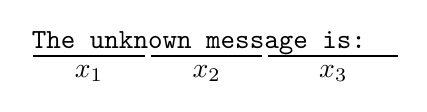
\begin{tikzpicture}[x=0.75pt,y=0.75pt,yscale=-1,xscale=1]
%uncomment if require: \path (0,40); %set diagram left start at 0, and has height of 40

%Straight Lines [id:da041820242795031604] 
\draw    (4,16) -- (58,16) ;
%Straight Lines [id:da47747795120640646] 
\draw    (61,16) -- (114.5,16) ;
%Straight Lines [id:da2450028819137724] 
\draw    (117.5,16) -- (180,16) ;

% Text Node
\draw (2,3) node [anchor=north west][inner sep=0.75pt]   [align=left] {
\texttt{The unknown message is:}
};
% Text Node
\draw (31,19.4) node [anchor=north] [inner sep=0.75pt]    {$x_{1}$};
% Text Node
\draw (87.75,19.4) node [anchor=north] [inner sep=0.75pt]    {$x_{2}$};
% Text Node
\draw (148.75,19.4) node [anchor=north] [inner sep=0.75pt]    {$x_{3}$};


\end{tikzpicture}